\section{Data management}
\begin{flushright}
\textit{No problem is too small or too trivial if we can really do something about it.} \\
-- Richard Feynman 
\end{flushright}


Digital data and associated software are critical MSL assets. Like any other assets, they should be cared for and maintained. This section is about data management planning. 

\subsection{Data management planning}
MSL should identify its requirements for data management so that implementations (specific procedures as well as supporting IT services) can be evaluated. 

A Data Management Plan (DMP) describes how data is managed, from initial production, through data processing to, finally, long-term storage. It should cover how data is handled, who is responsible, and how adherence to the plan will be monitored.

The DMP should contain sufficient detail to enable stakeholders (MSL staff, managers, and IT support) to understand the requirements for data management.

\subsubsection{Points to be considered in a data management plan}
\begin{enumerate}
 \item How is data generated? What software is used? 
 \item Data formats (e.g., raw text, .csv, .xlsx, XML, etc). 
 \item Is data annotated (with metadata)? Are standards used (which)? 
 \item Where is data stored? How is it organised (common file structure, database, etc)? 
 \item Size of data (storage and networking requirements)? 
 \item How is initial (raw) data secured? Level of protection required? 
 \item How is data processed? What software is used? 
 \item How is integrity maintained? Is there an audit trail?
 \item Do policies limit access to, and sharing of, (raw or processed) data? How are these policies implemented?
 \item How are final (published) reports and data related (records of processing, work flows, etc)?
 \item How is data, records of work flows, etc, archived? 
 \item How is software maintained (over time)?
 \item How long must data and software be retained?  
 \item Responsibilities for data (stewardship, custody)?\footnote{A `custodian`  is usually a manger with responsibility for the business function of data; they will have responsibility for planning and policy-making on data management. A `steward` is a subject-matter expert with responsibility for how data is used; they perform the work to manage data.}
 \item Who is responsible for the DMP (audits, reviews, etc)? 
\end{enumerate}

\subsubsection{17025 requirements}

All commercial calibration data, unless explicitly noted otherwise, will be confidential to MSL (17025 clause 4.2).

When technical records are in the form of electronic data, they shall be maintained according to 17025 clauses 7.1.

Electronic data management systems used by MSL shall comply with clauses 7.11 of the standard, which deals with control of data and information management.

The control of all records shall comply with clauses 8.4 of the standard, which deal with the control of records.

\subsubsection{Example: A DMP for RF standards}
\paragraph{Raw data} is produced by bespoke data acquisition software written in Python. A github repository is used to store this data on the corporate file server, which is cloned on lab and office machines. 

\paragraph{Data acquisition} software is developed under version control using a cloud-based repository (github). A record of the version(s) used during a job is logged when raw data is collected.  

\paragraph{The data formats} used are mainly: plain text files, spreadsheet files (.xls and.xlsx) and Python source (text files with extension .py). The text and Python files are largely for storing configuration information and metadata; spreadsheet files contain measurement data. Results of data processing are also generated in plain text and in spreadsheet files; there is also one proprietary binary file format used for some data (the GTC archive). 

Note, there are no spreadsheet software requirements. Spreadsheets containing data may used for \textit{ad hoc} calculations but the main data analysis is done in Python. 

No metadata standards are followed. 

\paragraph{Data is organised} in a hierarchy of sub-folders under a job-specific root folder; sub-folder names are generally composed of a time-stamp added to a descriptive root (e.g., Fig.~\ref{fig:runs} shows sub-folders where the `sp' stands for S-parameters). The results of data processing are stored in a similar way, using folder names that begin
with `dp' followed by a date and time stamp (see Fig.~\ref{fig:folders}) 

The storage requirement for a completed job is typically several megabytes.

\begin{figure}[ht]
 \centering
  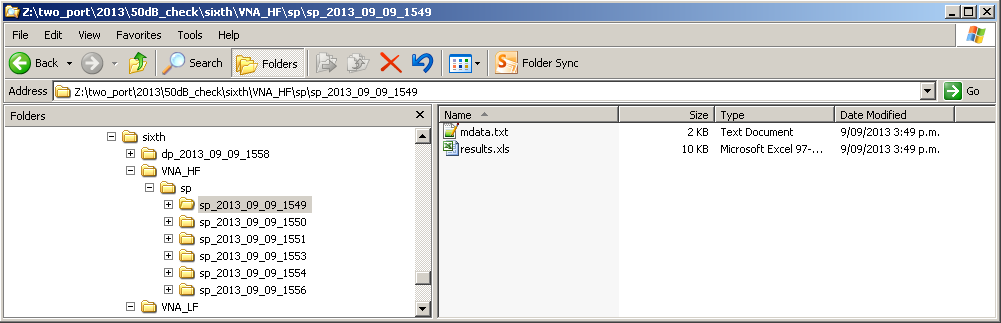
\includegraphics[width=0.8\linewidth]{pictures/filesystem_vna_runs.png}
  \caption{Measurement runs (sub-folders) inside an `sp' measurement folder (pane on the left) and the contents of one run folder (pane on the right).}
  \label{fig:runs}
\end{figure}

\begin{figure}[ht]
 \centering
  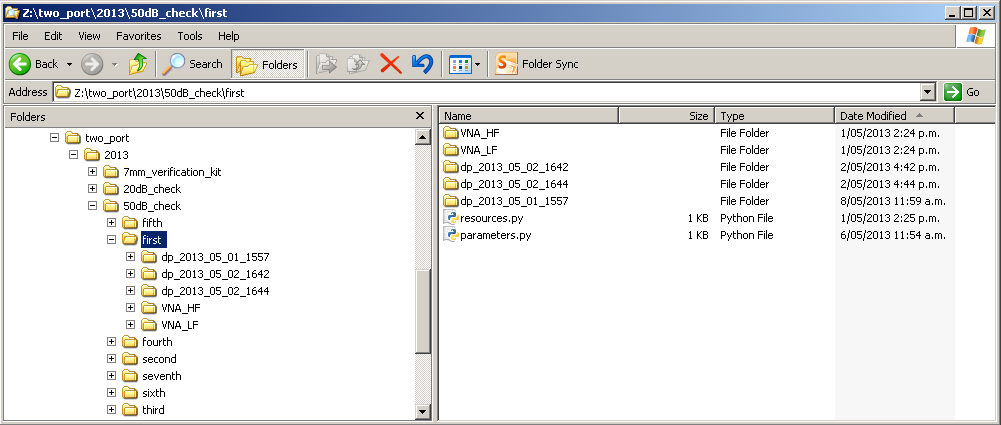
\includegraphics[width=0.8\linewidth]{pictures/filesystem_runs.png}
  \caption{View of a root folder structure for one job (the root is `first', organised below `two\_port', the year, and `50dB\_check'), containing three data processing sub-folders as well as VNA sub-folders in which raw data and configuration information is stored.}
  \label{fig:folders}
\end{figure}

\paragraph{Data integrity} is maintained by a git repository for each job. The initial job set-up creates a bare repository on the corporate file server (I-drive), which is immediately cloned to the lab computer. After raw data has been collected, it is committed to the local repository by the metrologist and a copy is pushed to the I-drive. 

This produces a (complete and independent) lab copy of the data and a remote copy on the I-drive; the I-drive is also routinely backed up by IT service (24-hour cycle). 

Using a repository guards against unintended accidental changes to data and also guards against intermittent network problems, by allowing work to be carried out locally until network access is restored.

\paragraph{All data} collected in commercial jobs is confidential to MSL by default. So, the `private' I-drive allocated to MSL is used, which restricts access to MSL staff. No other privacy protections are necessary.  

\paragraph{Data is processed} by bespoke Python software (also version-controlled) and the results stored in the same folder structure (see Fig.~\ref{fig:folders}). This allows the git repository to capture all stages of analysis. Using a git repository also facilitates review of processing details at a later date, or independent processing on the data without loss of information obtained earlier. 

When final client-specific analysis steps are required, the Python script for these last steps will be stored in the section file system commercial job file, which is separately located on the I-drive. The final report is also saved in this commercial job file. 

\paragraph{On completion} of a job, the repository is left undisturbed on local computers and on the corporate file server. There is no specific `archiving' process. The amount of data does not warrant compression and any eventual future analysis will be facilitated by maintaining the local file structure. 

Data and software must be retained indefinitely. 

The reliance on open-source Python software will help to provide on-going access to the functionality of our software. Python, of course, evolves and regular upgrades are expected. A suite of unit-test cases are used to facilitate migration and acceptance-testing of new versions.

\paragraph{Responsibilities} for data relate to custody and stewardship. The MSL Director is the nominally the custodian of data, but this is delegated to the Team Manager in charge of the section. The data stewards are MSL staff  qualified for the measurement procedure (MSL Competency Matrix). 

Adherence to the DMP will be reviewed annually and a record of review kept in the section files (lab book). 
